% !TEX root = ../../../main.tex
% 来源：中学数学实验教材·第二册（几何）
% 章节：圆 / 圆的基本性质
% 原始文件：4.tex，行 211-218
% 类型：tikz
% ---
		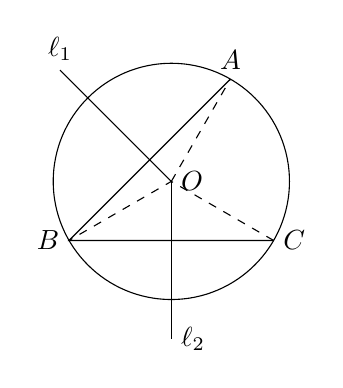
\begin{tikzpicture}[>=latex, scale=1]
\draw (0,0)node[right]{$O$} circle (1.5);
\draw[dashed] (-30:1.5)node[right]{$C$}--(0,0)--(-150:1.5)node[left]{$B$};
\draw (-30:1.5)--(-150:1.5)--(60:1.5);
\draw[dashed] (0,0)--(60:1.5)node[above]{$A$};
\draw (0,0)--(-90:2)node[right]{$\ell_2$};
\draw (0,0)--(135:2)node[above]{$\ell_1$};
		\end{tikzpicture}
